\documentclass[a4paper, 12pt]{extreport}

\usepackage{dp}
\usepackage{fancyhdr}
\usepackage{setspace}
\usepackage[Glenn]{fncychap}
%Options: Sonny, Lenny, Glenn, Conny, Rejne, Bjarne, Bjornstrup
\usepackage{hyperref}

\newcommand{\latex}{\LaTeX{}}
\newcommand{\stylecolor}{\color{astral}} % choose the color  added <<<<
\ChNameVar{\stylecolor\Large\fontfamily{put}\selectfont}

\newlength{\beforechapter}
\newlength{\afterchapter}

\setlength{\beforechapter}{-3\baselineskip} % substract some space before the chapter title <<<<<<
\setlength{\afterchapter}{2\baselineskip} % add space after chapter title   <<<<<<<<<<<<<

\makeatletter % added <<<
\def\mghrulefill#1{\stylecolor\leavevmode\leaders\hrule\@height #1\hfill\kern\z@}
  \renewcommand{\DOCH}{%
    \settoheight{\myhi}{\CTV\FmTi{Test}}
    \setlength{\py}{\baselineskip}
    \addtolength{\py}{\RW}
    \addtolength{\py}{\myhi}
    \setlength{\pyy}{\py}
    \addtolength{\pyy}{-1\RW}
    \vskip \beforechapter
    \raggedright
    \CNV\FmN{\@chapapp}\space\CNoV\thechapter
    \hskip 3pt\mghrulefill{\RW}\rule[-1\pyy]{2\RW}{\py}\par\nobreak}


  \renewcommand{\DOTI}[1]{%
    \addtolength{\pyy}{-4pt}
    \settoheight{\myhi}{\CTV\FmTi{#1}}
    \addtolength{\myhi}{\py}
    \addtolength{\myhi}{-1\RW}
    \vskip -1\pyy
    \rule{2\RW}{\myhi}\mghrulefill{\RW}\hskip 2pt
    \raggedleft\CTV\FmTi{#1}\par\nobreak
    \vskip \afterchapter
}


\def\@makeschapterhead#1{%
    \vspace*{50\p@}%
    \vskip \beforechapter
    {\parindent \z@ \raggedright
        \normalfont
        \interlinepenalty\@M
        \DOTIS{#1}
        \vskip -40\p@
        \vskip \afterchapter}
    }
\makeatother

\renewcommand{\chaptermark}[1]{%
  \markboth{#1}{}}

\lhead{\scriptsize\slshape\nouppercase{\leftmark}}
\rhead{\scriptsize\slshape(Quase) Todo semestre de Cálculo}

\pagestyle{fancy}

\hypersetup{
    colorlinks=true,
    linktocpage=true,
    linkcolor=astral,
    filecolor=magenta,
    urlcolor=astral,
    unicode=true,
    pdftitle={(Quase) Todo semestre de Cálculo - 2ªed},
    pdfpagemode=FullScreen,
    pdfauthor={rasteli}
}

\graphicspath{{./Images/}}

\def\doctitle{(Quase) Todo semestre de Cálculo}
\def\docauthor{Rasteli}

\title{\doctitle}
\author{\docauthor}

\begin{document}
  \selectlanguage{portuguese}
  %\maketitle

  \begin{titlepage}
	  \centering
    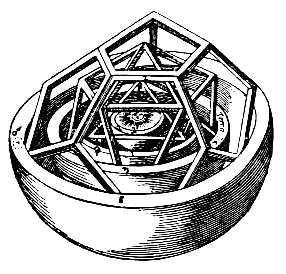
\includegraphics[width=0.15\textwidth]{geoart}\par\vspace{1cm}
	  \vspace{1.5cm}
	  {\huge\bfseries \doctitle\par}
	  \vspace{1cm}
    {\Large {Pequeno estudo sobre a maioria dos tópicos abordados durante o semestre do curso de cálculo II}\par}
	  \vspace{1cm}
	  {\Large\itshape \docauthor\par}

	  \vfill

  % Bottom of the page
	  {\large \today\par}
  \end{titlepage}
  \tableofcontents

  \newpage

  \chapter{Área entre funções}
    De fato, quando integra-se uma função num intervalo $ [a, b] $, obtém-se a área da região sob esta função no dado intervalo.
    Seja $ f $ uma função contínua em $ I $ tal que $ I \supseteq [a, b] $, a área $ A $ da região sob $ f $ em $ [a, b] $ é dada por

    \begin{equation}
      A = \int_a^b{f(x)}\diff x
    \end{equation}

    De modo similar, sejam $ f $ e $ g $ funções contínuas em $ I $ tal que $ I \supseteq [a, b] $ e $ f(x) \geqslant g(x) $, a área $ A $ da região entre
    $ f $ e $ g $ em $ [a, b] $ é dada por

    \begin{equation}
      A = \int_a^b{[f(x) - g(x)]}\diff x
    \end{equation}

    \begin{center}
      {
        (1.1)
        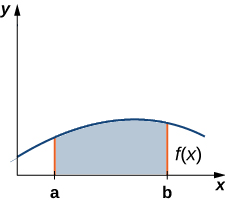
\includegraphics{fx}
      }
      \ \ \ \ \ \ \ \ \ \ \ \ \
      {
        (1.2)
        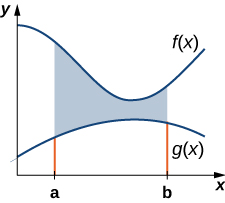
\includegraphics{two-func}
      }
    \end{center}

    Entretanto, para funções $ f $ e $ g $ que se intersectam no intervalo de interesse $ (a, b) $, a área $A$ da região entre elas \textbf{delimitada pelas
    retas} $x=a$ e $x=b$ é dada por

    \begin{equation} \label{eq:3}
      A = \int_a^b{|f(x) - g(x)|}\diff x
    \end{equation}

    \flushleft porém cada caso pode requerir sua própria estratégia.

    {\justifying É importante frisar que, caso a região cuja área deve ser calculada esteja abaixo do eixo de referência,
    a área $A$ é a integral negativa.}

    \subsection*{\small {\color{astral}EXEMPLO 1} \textmd{
      Considere a função $f(x) = \sqrt{x}$. Encontre a área da região delimitada pela função e pelas retas $x=5$ e $x=20$.
    }}
      Sabemos que a área $A=\int_a^b{f(x)dx}$, $f(x)=\sqrt{x}$ e $[a, b]=[5, 20]$, então
      $$ A = \int_5^{20}{\sqrt{x}\diff x} = \frac{14\sqrt{125}}{3}\mathrm{u^2} $$
      \qed{astral}

    \subsection*{\small {\color{astral}EXEMPLO 2} \textmd{
      Considere as funções $f(x) = 9-\left(\frac{x}{2}\right)^2$ e $g(x) = 6-x$. Encontre a área da região delimitada pelas funções.
    }}
      Como nenhum intervalo de integração foi dado, consideremos os pontos de intersecção.
        \begin{equation*}
          \begin{split}
            f(x) & = g(x) \\
            9-\left(\frac{x}{2}\right)^2 & = 6-x \\
            3+x-\frac{x^2}{4} & = 0 \\
            x^2-4x-12 & = 0
          \end{split}
        \end{equation*}
      Resolvendo esta equação de 2° grau, concluímos que $f(x)$ e $g(x)$ se intersectam em $x = -2$ e $x = 6$. Logo, estes compõem o intervalo.

      Faça o gráfico:

      \begin{center}
        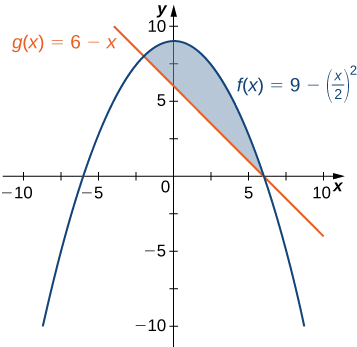
\includegraphics{eg2}
      \end{center}

      Perceba que $f(x) \geqslant g(x)$ em $[-2, 6]$, portanto a área
      \begin{equation*}
        \begin{split}
          A & = \int_{-2}^6{[f(x)-g(x)]\diff x} \\
            & = \int_{-2}^6{\left[9-\left(\frac{x}{2}\right)^2-(6-x)\right]\diff x} \\
            & = \int_{-2}^6{\left(3+x-\frac{x^2}{4}\right)\diff x} \\
            & = \frac{64}{3}\mathrm{u^2}
        \end{split}
      \end{equation*}
      \qed{astral}

    \subsection*{\small {\color{astral}EXEMPLO 3} \textmd{
      Considere as funções $f(x) = \sin(x)$ e $g(x) = \cos(x)$. Encontre a área entre as funções no intervalo $[0, \pi]$.
    }}
      O gráfico com as duas funções é o que segue:
      \begin{center}
        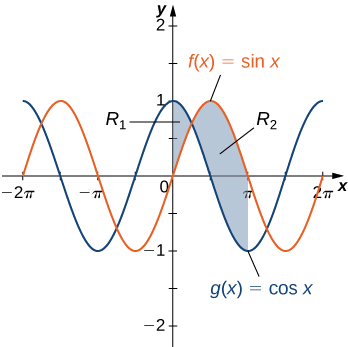
\includegraphics{eg3}
      \end{center}
      \justifying
      Perceba que a região cuja área foi requisitada não é única, mas composta por duas subregiões ($R_1$ e $R_2$). Isto é devido
      a não existir uma função que seja maior por todo o intervalo. Na verdade, para $x\in[0, \frac{\pi}{4}]$, $g(x) \geqslant f(x)$. E, para
      $x\in[\frac{\pi}{4}, \pi]$, $f(x) \geqslant g(x)$\footnote{
        $\frac{\pi}{4}$ é a abscissa da intersecção das funções no intervalo $(0, \pi)$.
        É onde $f$ sobrepassa $g$ em $x$.
      }.

      A fórmula em (\ref{eq:3}) parece resolver este problema, pois as funções se cruzam no intervalo $(0, \pi)$ e a área entre elas está, de fato,
      delimitada pelas retas $x = 0$ e $x = \pi$. Então

      \begin{equation*}
        A = \int_0^\pi{|f(x) - g(x)|}\diff x
      \end{equation*}
      mas $|f(x) - g(x)| = |\sin(x) - \cos(x)|$ e, para $x\in[0, \frac{\pi}{4}]$, $g(x) \geqslant f(x)$, então
      \begin{equation*}
        |\sin(x) - \cos(x)| = \cos(x) - \sin(x)
      \end{equation*}
      e, para $x\in[\frac{\pi}{4}, \pi]$, $f(x) \geqslant g(x)$, então
      \begin{equation*}
        |\sin(x) - \cos(x)| = \sin(x) - \cos(x)
      \end{equation*}
      Portanto
      \begin{equation*}
        \begin{split}
          A & = \int_0^\pi{|\sin(x) - \cos(x)|\diff x} \\
            & = \int_0^\frac{\pi}{4}{[\cos(x) - \sin(x)]\diff x} + \int_{\frac{\pi}{4}}^\pi{[\sin(x) - \cos(x)]\diff x} \\
            & = (\sqrt{2} - 1) + (\sqrt{2} + 1) = 2\sqrt{2}\mathrm{u^2}
        \end{split}
      \end{equation*}
      \qed{astral}

    \subsection*{\small {\color{astral}EXEMPLO 4} \textmd{
      Considere as funções $f(x) = \sqrt{x}$ e $g(x) = \frac{3}{2}-\frac{x}{2}$. Encontre a área entre as funções em $[0, 3]$.
    }}
    \noindent
      Tal é o gráfico:
      \begin{center}
        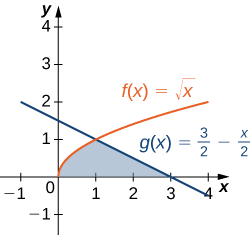
\includegraphics{eg4}
      \end{center}
      Tentemos algo diferente: integrar em relação a $y$. De fato, é mais fácil calcular a área em termos de $y$, pois só precisamos
      resolver uma integral.

      \vspace{5mm}

      \noindent Seja $y = f(x)$ e $x = v(y)$, então $v(y) = y^2$ e seja $y = g(x)$ e $x = w(y)$, então $w(y) = 3 - 2y$. Note que o intervalo de interesse agora
      é $[0, 1]$ no eixo $y$, pois redefinimos as funções em termos de $y$, portanto $w(y) \geqslant v(y)$ em $[0, 1]$.
      Podemos aplicar (2), pois todas nossas formulações ainda se mantêm. Então
      \begin{equation*}
        \begin{split}
          A & = \int_0^1{[w(y)-v(y)]\diff y} \\
            & = \int_0^1{(3-2y-y^2)\diff y} \\
            & = \frac{5}{3}\mathrm{u^2}
        \end{split}
      \end{equation*}
      \qed{astral}

    \section{Exercícios}
      \begin{enumerate}
        \item Considere as funções $f(x) = x^2-2x$ e $g(x) = x$. Encontre a área delimitada pelas funções.
        \item Considere as funções $f(x) = x^2$ e $g(x) = 2-x$. Determine a área delimitada pelas funções e pelas retas $x = 0$ e $x = 2$.
        \item Considere as funções $f(x) = x+2$ e $g(x) = \sqrt{-x}$. Encontre a área delimitada pelas funções em $[-2, 0]$ e pelo eixo $x$.
          Faça em termos de $x$ e em termos de $y$.
        \item Cada uma das regiões $A$, $B$ e $C$ delimitadas por $f$ e pelo eixo $x$ tem área 3. Determine o valor de
          $$ \int_{-4}^2{[f(x)+2x+5]dx} $$
        \begin{center}
          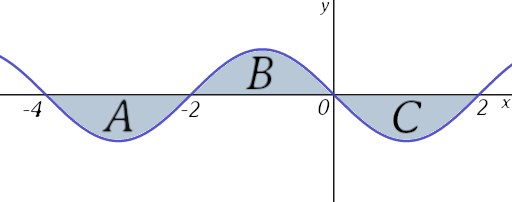
\includegraphics[scale=0.35]{ex4}
        \end{center}
      \end{enumerate}

  \chapter{Integração por frações parciais}
    A técnica de integração por frações parciais consiste em expressar uma integral de uma função racional (divisão de polinômios)
    como uma integral da soma de frações mais simples, \textsl{frações parciais}, que sabemos integrar. Como exemplo, se levarmos as frações
    $\frac{2}{x-1}$ e $\frac{1}{x+2}$ a um denominador comum, temos

    $$ \frac{2}{x-1} - \frac{1}{x+2} = \frac{2(x+2)-(x-1)}{(x-1)(x+2)} = \frac{x+5}{x^2+x-2}$$
    Revertendo o procedimento, vemos como integrar a função:

    $$ \int{\frac{x+5}{x^2+x-2}\diff x} = \int{\left(\frac{2}{x-1} - \frac{1}{x+2}\right)\diff x} = 2\ln|x-1| - \ln|x+2| + C $$

    Consideremos a função racional

    \begin{equation}
      f(x) = \frac{P(x)}{Q(x)}
    \end{equation}
    onde $P$ e $Q$ são polinômios e um polinômio qualquer $A(x) = a_nx^n + a_{n-1}x^{n-1} + \cdots + a_1x + a_0$, então, se $a_n \neq 0$, dizemos que o grau de $A$
    é $n$ e escrevemos $gr(A) = n$. É possível expressar $f$ como a soma de frações mais simples se $gr(P) < gr(Q)$. Então $f$ é chamada \textsl{própria}.

    Se $f$ for \textsl{imprópria}, isto é, $gr(P) \geqslant gr(Q)$, devemos antes dividir $P$ por $Q$ (divisão de polinômios) até um resto $R(x)$ tal que $gr(R) < gr(Q)$. Então $f$ pode ser expressa como

    \begin{equation}
      f(x) = \frac{P(x)}{Q(x)} = S(x) + \frac{R(x)}{Q(x)}
    \end{equation}
    onde $S$ e $R$ também são polinômios. A seguir, no exemplo, vemos que, por vezes, esta etapa preliminar é tudo de que precisamos.

    \subsection*{\small {\color{astral}EXEMPLO 1} \textmd{Determine \large$\int{\frac{x^3+x}{x-1}}$\normalsize$\diff x$}}
      Note que o grau do numerador é maior que o grau do denominador, então devemos primeiro realizar a divisão.
      \begin{center}
        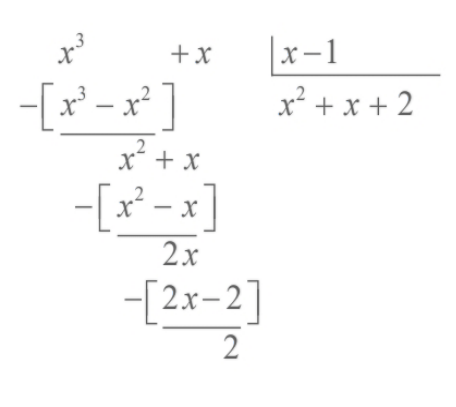
\includegraphics[scale=0.25]{poly-div}
      \end{center}
      Concluímos que
      \begin{equation*}
        \begin{split}
          \int{\frac{x^3+x}{x-1}\diff x} & = \int{\left(x^2+x+2+\frac{2}{x-1}\right)\diff x} \\
                                    & = \frac{x^3}{3} + \frac{x^2}{2} + 2x + 2\ln|x-1| + C
        \end{split}
      \end{equation*}
      \qed{astral}

    Quando $Q(x)$ é fatorável, o próximo passo é fatorá-lo tanto quanto possível. Devemos ser capazes de fatorá-lo como um produto
    de fatores lineares (da forma $ax + b$) e fatores quadráticos irredutíveis (da forma $ax^2 + bx + c$, onde $b^2 - 4ac < 0$).
    Por exemplo, seja $Q(x) = x^4-16$, pode ser fatorado como $$ Q(x) = (x^2-4)(x^2+4) = (x-2)(x+2)(x^2+4) $$

    O terceiro passo consiste em expressar a função racional própria $\frac{R(x)}{Q(x)}$ em uma soma de frações parciais da forma
    $$\frac{A}{ax+b} \ \ \textup{ou} \ \ \frac{Ax+B}{ax^2+bx+c}$$

    \vspace{10mm}
    \subsection*{\small CASO I $\mathbf{Q(x)}$ é um produto de fatores lineares distintos}
      \flushleft Isto é, $$ Q(x) = (a_1x + b_1)(a_2x + b_2)\cdots(a_kx + b_k) $$ onde nenhum fator é repetido. Portanto existem constantes
      $A_1, A_2,..., A_k$ tais que
      \begin{equation} \label{eq:r}
        \frac{R(x)}{Q(x)} = \frac{A_1}{a_1x+b_1} + \frac{A_2}{a_2x+b_2} + \cdots + \frac{A_k}{a_kx+b_k}
      \end{equation}

      \subsection*{\small {\color{astral}EXEMPLO 2} \textmd{Determine \large$\int{\frac{x^2+2x-1}{2x^3+3x^2-2x}}$\normalsize$\diff x$}}
        \justifying Não é necessário realizar divisão, pois o grau do numerador é menor que o grau do denominador. Primeiramente precisamos fatorar o denominador
        $$ 2x^3+3x^2-2x = x(2x^2+3x-2) = x(2x-1)(x+2) $$
        Em seguida, decompomos o integrando em frações parciais
        $$ \frac{x^2+2x-1}{x(2x-1)(x+2)} = \frac{A}{x} + \frac{B}{2x-1} + \frac{C}{x+2} $$

        Para obtermos os valores de $A$, $B$ e $C$, multiplicamos toda a equação pelo mínimo múltiplo comum dos denominadores, $x(2x-1)(x+2)$
        $$ x^2+2x-1 = A(2x-1)(x+2) + Bx(x+2) + Cx(2x-1) $$
        Expandindo os termos e evidenciando os fatores comuns do lado direito da equação, temos
        $$ x^2+2x-1 = (2A+B+2C)x^2 + (3A+2B-C)x - 2A $$

        Ora, isto é uma equação, portanto, o polinômio do lado esquerdo é idêntico ao polinômio do lado direito. Isto quer dizer que os coeficientes
        de fatores correspondentes devem ser iguais. Do lado esquerdo, o coeficiente de $x^2$ é $1$; do lado direito, $2A+B+2C$, ou seja, $2A+B+2C = 1$.
        Do mesmo modo, os coeficientes de $x$ e os termos constantes são iguais. Obtemos, então, o sistema
        \begin{equation*}
          \begin{cases}
            2A+B+2C = 1 \\
            3A+2B-C = 2 \\
            2A = 1
          \end{cases}
        \end{equation*}
        Resolvendo, obtemos $A = \frac{1}{2}$, $B = \frac{1}{5}$ e $C = -\frac{1}{10}$. Assim
        \begin{equation*}
          \begin{split}
            \int{\frac{x^2+2x-1}{2x^3+3x^2-2x}\diff x} & = \int{\left(\frac{1}{2x} + \frac{1}{5(2x-1)} - \frac{1}{10(x+2)}\right)\diff x} \\
                                                  & = \frac{1}{2}\ln|x| + \frac{1}{10}\ln|2x-1| - \frac{1}{10}\ln|x+2| + K
          \end{split}
        \end{equation*}
        \qed{astral}

        \subsection*{\color{coverup}\small MÉTODO DA COBERTURA (COVER-UP)}
          O método da cobertura consiste em descobrir os termos dos numeradores das frações parciais de uma função racional própria multiplicando
          a equação (\ref{eq:r}) pelo denominador da fração cujo numerador contém o termo a ser obtido. Em seguida, atribui-se um valor a $x$ de modo que
          a equação possa ser simplificada, onde a única incógnita é o termo a ser obtido.
          Por exemplo, considere $$ \frac{x+3}{x^2-4} = \frac{x+3}{(x-2)(x+2)} = \frac{A}{x-2} + \frac{B}{x+2} $$
          Para obtermos o valor de $A$, multiplicamos a equação por $x-2$, seu denominador, obtendo
          $$ \frac{x+3}{x+2} = A + \frac{B}{x+2}(x-2) $$
          Perceba que $x-2$ é um fator de {\large$\frac{B}{x+2}$}, portanto, se $x=2$, todo o termo resulta em $0$, restando
          $$ A = \frac{2+3}{2+2} = \frac{5}{4} $$
          Do mesmo modo, para obtermos B, multiplicamos a equação por $x+2$, obtendo
          $$ \frac{x+3}{x-2} = \frac{A}{x-2}(x+2) + B $$
          Se $x = -2$, então
          $$ B = \frac{-2+3}{-2-2} = -\frac{1}{4} $$

          Saiba, entretanto, que este método não é infalível. Para ilustrarmos esta tragédia, consideremos a seguinte função racional própria
          $$ f(x) = \frac{x^2+2x+3}{x^4-16} $$
          Devemos fatorar o denominador. Então obtemos
          $$ f(x) = \frac{x^2+2x+3}{(x-2)(x+2)(x^2+4)} $$
          \vspace{1mm}
          Decompondo a função em frações parciais
          $$ f(x) = \frac{x^2+2x+3}{(x-2)(x+2)(x^2+4)} = \frac{A}{x-2} + \frac{B}{x+2} + \frac{Cx+D}{x^2+4} $$
          \vspace{1mm}
          Perceba que o denominador $x^2+4$ é quadrático, portanto um linear ($Cx+D$, nesse caso) deve ser o numerador.
          Suponha que queiramos obter o valor de $C$ ou $D$, multiplicaríamos a equação por seu denominador, a saber, $x^2+4$, que resulta em
          $$ \frac{x^2+2x+3}{(x-2)(x+2)} = \frac{A}{x-2}(x^2+4) + \frac{B}{x+2}(x^2+4) + Cx+D $$
          \vspace{1mm}
          Veja que $\forall x, x^2+4 > 0$ (lê-se "para todo valor de $x$, $x^2+4$ é sempre maior que $0$"), portanto não conseguimos simplificar a
          equação para $C$ ou $D$ (para $A$ e $B$, cobertura ainda funciona).

    \vspace{10mm}
    \subsection*{\small CASO II $\mathbf{Q(x)}$ é um produto de fatores lineares, alguns dos quais se repetem}
      Suponha que o \textsl{k}-ésimo fator linear $a_kx+b_k$ seja repetido $r$ vezes, isto é, $(a_kx+b_k)^r$ ocorre em $Q(x)$. Então precisaríamos, como chamo,
      construir a potência, de modo que o termo com tal fator seja decomposto em
      $$ \frac{A_k}{a_kx+b_k} + \frac{A_{k+1}}{(a_kx+b_k)^2} + \cdots + \frac{A_{k+r-1}}{(a_kx+b_k)^r} $$

      \subsection*{\small {\color{astral}EXEMPLO 3} \textmd{Determine \large$\int{\frac{x^4-2x^2-4x+1}{x^3-x^2-x+1}}$\normalsize$\diff x$}}
        O primeiro passo é dividir $P(x) = x^4-2x^2-4x+1$ por $Q(x)= x^3-x^2-x+1$, pois $gr(Q) < gr(P)$. O resultado desta divisão é

        $$ \frac{x^4-2x^2-4x+1}{x^3-x^2-x+1} = x+1-\frac{4x}{x^3-x^2-x+1} $$

        \vspace{3mm}
        \noindent O segundo passo é fatorar $Q(x)$. Como $Q(1) = 0$, $x-1$ é um fator e, por divisão, encontramos o outro. Então
        \begin{equation*}
          \begin{split}
            x^3-x^2-x+1 & = (x-1)(x^2-1) = (x-1)(x-1)(x+1) \\
                        & = (x+1)(x-1)^2
          \end{split}
        \end{equation*}
        Como $x-1$ ocorre duas vezes, a decomposição em frações parciais é

        $$ \frac{4x}{(x+1)(x-1)^2} = \frac{A}{x-1} + \frac{B}{(x-1)^2} + \frac{C}{x+1} $$

        \vspace{3mm}
        \noindent Por cobertura, obtemos $B=2$ e $C=-1$. Para $A$, multiplicamos a equação pelo m.m.c. dos denominadores e substituímos os
        valores de $B$ e $C$, obtendo
        \begin{equation*}
          \begin{split}
            4x & = A(x+1)(x-1) + 2(x+1) - (x-1)^2 \\
            4x & = Ax^2-A + 2x+2 - x^2+2x-1 \\
            4x & = (A-1)x^2 + 4x - A + 1
          \end{split}
        \end{equation*}
        Então $A-1 = 0$, $\therefore A = 1$. Voltando à integral, temos
        \begin{equation*}
          \begin{split}
            \int{\frac{x^4-2x^2-4x+1}{x^3-x^2-x+1}\diff x} & = \int{\left\{x+1-\left[\frac{1}{x-1} + \frac{2}{(x-1)^2} - \frac{1}{x+1}\right]\right\}\diff x} \\
                                                      & = \frac{x^2}{2}+x-\ln|x-1|+\frac{2}{x-1}+\ln|x+1| + K \\
                                                      & = \frac{x^2}{2}+x+\frac{2}{x-1}+\ln\left|\frac{x+1}{x-1}\right| + K
          \end{split}
        \end{equation*}
        \qed{astral}

    \section{Exercícios}
      {\color{astral}\textbf{1-6}} Calcule as integrais:
      \begin{multicols}{3}
        \begin{enumerate}
          \item \Large$\int{\frac{x-12}{x^2-4x}}$\normalsize\textit{dx}
          \item \Large$\int{\frac{5}{x^2+3x-4}}$\normalsize\textit{dx}
          \item \Large$\int_{\scalebox{0.5}{-1}}^{\scalebox{0.5}0}{\frac{x^3-4x+1}{x^2-3x+2}}$\normalsize\textit{dx}
          \item \Large$\int{\frac{1}{y(y-a)}}$\normalsize\textit{dy}
          \item \Large$\int_{\scalebox{0.5}1}^{\scalebox{0.5}2}{\frac{x^3+4x^2+x-1}{x^3+x^2}}$\normalsize\textit{dx}
          \item \Large$\int{\frac{1}{(t^2-1)^2}}$\normalsize\textit{dt}
        \end{enumerate}
      \end{multicols}

  \chapter{Funções multivariáveis e derivadas parciais}
    Uma função $f$ de várias variáveis é uma relação onde cada ênupla ordenada (par, tripla, quádrupla \textit{etc}) de números reais $(x_1, x_2, ..., x_n)$
    de um conjunto $D \subset \mathbb{R}^n$ associa-se a um único número real, denotado por $f(x_1, x_2, ..., x_n)$. Diz-se que $D$ é o domínio de $f$
    e sua imagem é o conjunto de valores possíveis de $f$, isto é, $\{f(x_1, x_2, ..., x_n) | (x_1, x_2, ..., x_n) \in D\}$. Por exemplo, se representarmos
    o domínio $D$ como um subconjunto de um plano $xy$, a imagem será um conjunto de números na reta real, representada pelo eixo $z$.

    A derivada de $f$, diferentemente da diferenciação implícita, onde consideramos cada variável como uma função, é em relação a uma de suas variáveis, onde
    todas as outras são consideradas constantes. Esta derivada é denominada \textsl{parcial}.

    Considere uma função $f$ de duas variáveis $x$ e $y$ e suponha que deixemos só $x$ variar e mantemos fixa $y$. Consideramos, então,
    uma função de uma única variável, $g(x) = f(x, y)$. A derivada de $g$ é, portanto, a derivada parcial de $f$ em relação a $x$ e a
    denotaremos por $\frac{\partial}{\partial x}f(x, y)$. Pela definição de derivada, temos
    $$ \frac{d}{dx}g(x) = \lim_{h \to 0}{\frac{g(x+h) - g(x)}{h}} $$
    Portanto
    $$ \frac{\partial}{\partial x}f(x, y) = \lim_{h \to 0}{\frac{f(x+h, y) - f(x, y)}{h}} $$

    De modo similar, deixemos agora que somente $y$ varie. Assim $g(y) = f(x, y)$ e dizemos que a derivada de $g$ é a derivada parcial de $f$ em relação a $y$,
    denotada por $\frac{\partial}{\partial y}f(x, y)$. Temos
    $$ \frac{d}{dy}g(y) = \lim_{h \to 0}{\frac{g(y+h) - g(y)}{h}} $$
    Então
    $$ \frac{\partial}{\partial y}f(x, y) = \lim_{h \to 0}{\frac{f(x, y+h) - f(x, y)}{h}} $$

    De modo geral, se $u$ é uma função de $n$ variáveis, isto é, $u=f(x_1,...,x_n)$, sua derivada em relação a \textsl{i}-ésima variável $x_i$ é
    $$ \frac{\partial u}{\partial x_i} = \lim_{h \to 0}{\frac{f(x_1,..., x_{i-1}, x_i+h, x_{i+1},..., x_n) - f(x_1,...,x_i,...,x_n)}{h}} $$

    \subsection*{\color{coverup}\small OBSERVAÇÃO}
      Existe uma miríade de notações para uma derivada parcial. Abaixo estão escritas algumas considerando $z = f(x, y)$.
      $$ f_x(x, y) = f_x = \frac{\partial f}{\partial x} = \frac{\partial}{\partial x}f(x, y) = \partial_xf = \partial_xf(x, y) = \frac{\partial z}{\partial x} = f_1 = D_1f = D_xf$$
      $$ f_y(x, y) = f_y = \frac{\partial f}{\partial y} = \frac{\partial}{\partial y}f(x, y) = \partial_yf = \partial_yf(x, y) = \frac{\partial z}{\partial y} = f_2 = D_2f = D_yf$$

    \subsection*{\small {\color{astral}EXEMPLO 1} \textmd{Seja $f(x,y)=x^3+x^2y^3-2y^2$, encontre $f_x(2,1)$ e $f_y(2,1)$.}}
      \flushleft Derivando em relação a $x$ e mantendo $y$ constante, temos
      \begin{equation*}
        \begin{split}
          f_x(x,y) & = 3x^2 + 2xy^3 \\
          f_x(2,1) & = 3\cdot2^2 + 2\cdot2\cdot1^3 = 16
        \end{split}
      \end{equation*}

      \flushleft Derivando em relação a $y$ e mantendo $x$ constante, temos
      \begin{equation*}
        \begin{split}
          f_y(x,y) & = 3x^2y^2 - 4y \\
          f_y(2,1) & = 3\cdot2^2\cdot1^2 - 4\cdot1 = 8
        \end{split}
      \end{equation*}
      \qed{astral}

    \subsection*{\color{coverup}\small OBSERVAÇÃO}
      \justifying O que foi pedido no \textsl{Exemplo 1}, $f_x(2,1)$ e $f_y(2,1)$, é chamado gradiente de $f(2,1)$.
      Representado pelo símbolo $\nabla$ (\textsl{nabla}), o gradiente de uma função num ponto $p$ é um vetor que indica a direção de
      maior incremento de uma grandeza a partir de $p$ e cujo módulo é a taxa de incremento nessa direção e é dado por
      $$ \nabla f(p) = \left(\frac{\partial f(p)}{\partial x_1}, \frac{\partial f(p)}{\partial x_2},..., \frac{\partial f(p)}{\partial x_n}\right) $$
      No \textsl{Exemplo 1}, poderia ter sido pedido, de outra forma, $\nabla f(2,1)$.

      \subsection*{\small {\color{astral}EXEMPLO 2} \textmd{Seja $f(x,y,z)=e^{xy}\ln{z}$, determine $\nabla f(1,2,e)$.}}
        \flushleft Derivando em relação a $x$ e mantendo $y$ e $z$ constantes, temos
        \begin{equation*}
          \begin{split}
            f_x(x,y,z) & = ye^{xy}\ln{z} \\
            f_x(1,2,e) & = 2 \cdot e^2 \cdot \ln{e} = 2e^2
          \end{split}
        \end{equation*}

        \flushleft Derivando em relação a $y$ e mantendo $x$ e $z$ constantes, temos
        \begin{equation*}
          \begin{split}
            f_y(x,y,z) & = xe^{xy}\ln{z} \\
            f_y(1,2,e) & = 1 \cdot e^2 \cdot \ln{e} = e^2
          \end{split}
        \end{equation*}

        \flushleft Derivando em relação a $z$ e mantendo $x$ e $y$ constantes, temos
        \begin{equation*}
          \begin{split}
            f_z(x,y,z) & = \frac{e^{xy}}{z} \\
            f_z(1,2,e) & = \frac{e^2}{e} = e
          \end{split}
        \end{equation*}
        $\therefore \nabla f(1,2,e) = (2e^2, e^2, e)$
        \qed{astral}

    \subsection*{\color{coverup}\small DERIVADAS PARCIAIS DE ORDEM SUPERIOR}
      \justifying Se $f$ é uma função de $n$ variáveis, suas derivadas parciais $f_{x_1}$, $f_{x_2}$,\dots,$f_{x_n}$ também são funções de $n$ variáveis, de modo
      que podemos derivá-las parcialmente outra vez, chamadas \textsl{derivadas parciais de segunda ordem}, a que eu me refiro como $\textsl{dp}^2$
      (de modo geral, às \textsl{derivadas parciais de enésima ordem}, eu me refiro como $\textsl{dp}^n$). Se $z=f(x,y)$, denotamos suas $\textsl{dp}^2$, igualmente
      às $\textsl{dp}^1$, entre outras maneiras, por
      \begin{equation*}
        \begin{split}
          (f_x)_x = f_{xx} = f_{11} & = \frac{\partial}{\partial x}\left(\frac{\partial f}{\partial x}\right) = \frac{\partial^2f}{\partial x^2} = \frac{\partial^2z}{\partial x^2} = \partial_x\partial_xf \\
          \\
          (f_x)_y = f_{xy} = f_{12} & = \frac{\partial}{\partial y}\left(\frac{\partial f}{\partial x}\right) = \frac{\partial^2f}{\partial y\partial x} = \frac{\partial^2z}{\partial y\partial x} = \partial_y\partial_xf \\
          \\
          (f_y)_x = f_{yx} = f_{21} & = \frac{\partial}{\partial x}\left(\frac{\partial f}{\partial y}\right) = \frac{\partial^2f}{\partial x\partial y} = \frac{\partial^2z}{\partial x\partial y} = \partial_x\partial_yf \\
          \\
          (f_y)_y = f_{yy} = f_{22} & = \frac{\partial}{\partial y}\left(\frac{\partial f}{\partial y}\right) = \frac{\partial^2f}{\partial y^2} = \frac{\partial^2z}{\partial y^2} = \partial_y\partial_yf
        \end{split}
      \end{equation*}

      Saiba que a notação {\large$\sfrac{\partial^2f}{\partial y\partial x}$} ou $f_{xy}$ significa que primeiro devemos derivar parcialmente a função em relação a $x$ e,
      em seguida, em relação a $y$. {\large$\sfrac{\partial^2f}{\partial x\partial y}$} ou $f_{yx}$ significa o inverso.

      \subsection*{\small {\color{astral}EXEMPLO 3} \textmd{Determine todas as $\textsl{dp}^2$ de}}
        \vspace{-5mm}
        $$ f(x,y) = x^3 + x^2y^3 - 2y^2 $$
        No \textsl{Exemplo 1}, descobrimos que
        $$ f_x = 3x^2 + 2xy^3 \ \ \ \ \textup{e} \ \ \ \ f_y = 3x^2y^2 - 4y $$
        Logo
        \begin{multicols}{2}
          \noindent
          \begin{equation*}
            \begin{split}
              f_{xx} & = 6x + 2y^3 \\
              f_{yx} & = 6xy^2
            \end{split}
          \end{equation*}
          \begin{equation*}
            \begin{split}
              f_{xy} & = 6xy^2 \\
              f_{yy} & = 6x^2y - 4
            \end{split}
          \end{equation*}
        \end{multicols}
        \qed{astral}

        Observe que $f_{xy} = f_{yx}$ no \textsl{Exemplo 3}. Isto é verdade para a maioria das funções.
        O matemático francês Alexis Clairaut formulou um teorema que nos permite afirmar a igualdade $f_{xy} = f_{yx}$.

        \vspace{4mm}
        \noindent \fbox{
          \begin{minipage}{35em}
            \small
            {\color{infobox}Teorema de Clairaut} \normalfont Suponha que $f$ esteja definida em um disco $D$ que contenha
            o ponto $(a,b)$, isto é, $(a,b) \in D$. Se as funções $f_{xy}$ e $f_{yx}$
            forem ambas contínuas em $D$, então $f_{xy}(a,b) = f_{yx}(a,b)$.
          \end{minipage}
        }

      \subsection*{\small {\color{astral}EXEMPLO 4} \textmd{Seja $f(x,y,z) = \cos{(x+2yz)}$, calcule $f_{xxyz}$.}}
        \vspace{-8mm}
        \begin{equation*}
          \begin{split}
            f_x & = -\sin{(x+2yz)} \\
            f_{xx} & = -\cos{(x+2yz)} \\
            f_{xxy} & = 2z\sin{(x+2yz)} \\
            f_{xxyz} & = 4yz\cos{(x+2yz)} + 2\sin{(x+2yz)}
          \end{split}
        \end{equation*}
        \qed{astral}

      \section{Exercícios}
      {\color{astral}\textbf{1-2}} Encontre $f_x(x,y)$ e $f_y(x,y)$ utilizando a definição de derivadas parciais como limites e \hspace*{5mm} determine $\nabla f(1,-1)$.
        \begin{multicols}{2}
          \begin{enumerate}
            \item $f(x,y) =$ {\large$\frac{x}{y^2+x}$}
            \item $f(x,y) = 2x^2y - xy^2 + y$
          \end{enumerate}
        \end{multicols}
        {\color{astral}\textbf{3-8}} Determine \textbf{todas} as derivadas parciais de segunda ordem.
        \begin{multicols}{2}
          \begin{enumerate}
            \setcounter{enumi}{2}
            \item $f(x,y) = x^3y^5 + 2x^4y$
            \item $f(x,y) = \sin^2{(mx + my)}$
            \item $v =$ {\large$\frac{xy}{x-y}$}
            \item $z =$ {\large$\frac{x+y}{1-xy}$}
            \item $v = e^{xe^y}$
            \item $f(x,y) = \ln{(mxy+y^2)}$
          \end{enumerate}
        \end{multicols}
        {\color{astral}\textbf{9-12}} Verifique se as funções satisfazem o Teorema de Clairaut, isto é, se $z_{xy} = z_{yx}$.
        \begin{multicols}{2}
          \begin{enumerate}
            \setcounter{enumi}{8}
            \item $z = x^4y^3 - y^4$
            \item $z = \cos{(x^2y)}$
            \item $z = e^{xy}\sin{y}$
            \item $z = \ln{(x+2y)}$
          \end{enumerate}
        \end{multicols}


  \chapter{Integrais múltiplas}
    Seja $f$ uma função de duas variáveis definida em um retângulo fechado
    $$ R = [a,b] \times [c,d] = \left\{(x,y) \in \mathbb{R}^2 | a \leqslant x \leqslant b, c \leqslant y \leqslant d \right\} $$

    O gráfico de $f$ é a superfície de equação $z = f(x,y)$. Seja $f(x,y) \geqslant 0$ e $S$ o sólido acima da região $R$ e abaixo do gráfico de $f$, isto é,
    $$ S = \left\{(x,y,z) \in \mathbb{R}^3 | 0 \leqslant z \leqslant f(x,y), (x,y) \in R \right\} $$

    Concluímos que o volume $V$ de $S$, a partir de uma demonstração semelhante à integral unidimensional expressa como o valor limite da soma de Riemann, é
    $$ V = \iint_R{f(x,y)\diff A} = \lim_{m,n \to \infty}{\sum_{i=1}^m{\sum_{j=1}^n}{f(x_i,y_j)\Delta A}} $$
    onde $\Delta A = \Delta x\Delta y$.

    Usualmente calculamos uma integral dupla expressando-a como uma \textsl{integral iterada}, calculando duas integrais unidimensionais.
    Se integrarmos a função $f$ em relação a $y$ em $[c,d]$ mantendo $x$ constante, isto é, $\int_c^d{f(x,y)\diff y}$, obteremos um resultado dependente de $x$,
    portanto uma função de $x$:
    $$ \phi (x) = \int_c^d{f(x,y)\diff y} $$
    Em seguida, se integrarmos a função $\phi$ em relação a $x$ em $[a,b]$, obteremos
    \begin{equation} \label{eq:1}
      \int_a^b{\phi (x)\diff x} = \int_a^b{\left[\int_c^d{f(x,y)\diff y}\right]\diff x}
    \end{equation}

    A integral do lado direito de (\ref{eq:1}) é denominada \textsl{integral iterada}. Em geral, os colchetes são omitidos. Assim a integral
    \begin{equation}
      \int_a^b{\int_c^d{f(x,y)\diff y}\diff x} = \int_a^b{\left[\int_c^d{f(x,y)\diff y}\right]\diff x}
    \end{equation}
    indica que devemos primeiro integrar em relação a $y$ de $c$ até $d$, depois, em relação a $x$ de $a$ até $b$. Do mesmo modo, a integral
    \begin{equation}
      \int_c^d{\int_a^b{f(x,y)\diff x}\diff y} = \int_c^d{\left[\int_a^b{f(x,y)\diff x}\right]\diff y}
    \end{equation}
    indica que devemos primeiro integrar em relação a $x$ de $a$ até $b$, depois, em relação a $y$ de $c$ até $d$.

    \newpage

    \subsection*{\small {\color{astral}EXEMPLO 1} \textmd{Determine o valor das integrais iteradas}}
      \begin{multicols}{2}
        \begin{enumerate}
          \renewcommand{\theenumi}{(\alph{enumi})}
          \item $\int_0^3{\int_1^2{x^2y}\diff y}\diff x$
          \item $\int_1^2{\int_0^3{x^2y}\diff x}\diff y$
        \end{enumerate}
      \end{multicols}

      \noindent (a) Integramos primeiro em relação a $y$ mantendo $x$ constante
      $$ \int_1^2{x^2y}\diff y = \left[x^2\frac{y^2}{2}\right]_{y=1}^{y=2} = x^2\frac{2^2}{2} - x^2\frac{1^2}{2} = \frac{3}{2}x^2 $$
      Isto é, a função $\phi(x) = \frac{3}{2}x^2$. Agora integramos $\phi$ em relação a $x$ de $0$ a $3$
      \begin{equation*}
        \begin{split}
          \int_0^3{\int_1^2{x^2y}\diff y}\diff x & = \int_0^3{\left[\int_1^2{x^2y}\diff y\right]}\diff x \\
                                                 & = \int_0^3{\frac{3}{2}x^2}\diff x = \left[\frac{x^3}{2}\right]_{x=0}^{x=3} = \frac{27}{2}
        \end{split}
      \end{equation*}

      \noindent (b) Integramos primeiro em relação a $x$ mantendo $y$ constante
      \begin{equation*}
        \begin{split}
          \int_1^2{\int_0^3{x^2y}\diff x}\diff y & = \int_1^2{\left[\int_0^3{x^2y}\diff x\right]}\diff y = \int_1^2{\left[\frac{x^3}{3}y\right]_{x=0}^{x=3}}\diff x \\
                                                 & = \int_1^2{9y\hspace{1mm}\diff y} = \left[9\frac{y^2}{2}\right]_{y=1}^{y=2} = \frac{27}{2}
        \end{split}
      \end{equation*}
      \qed{astral}

      Semelhantemente ao teorema de Clairaut, o resultado das integrais no \textsl{Exemplo 1} foi o mesmo independentemente da ordem de integração.

        \vspace{4mm}
        \noindent \fbox{
          \begin{minipage}{35em}
            \small
            {\color{infobox}Teorema de Fubini} \normalfont Se $f$ for contínua no retângulo \\
            $R = \left\{(x,y) \in \mathbb{R}^2 | a \leqslant x \leqslant b, c \leqslant y \leqslant d \right\}$, então
            \vspace{-1mm}
            $$\iint_R{f(x,y)\diff A} = \int_a^b{\int_c^d{f(x,y)\diff y}\diff x} = \int_c^d{\int_a^b{f(x,y)\diff x}\diff y} $$

            De modo mais geral, esse resultado vale se supusermos que $f$ seja limitada em $R$, $f$ tenha descontinuidades apenas em um número
            finito de curvas suaves e que a integral iterada exista.
          \end{minipage}
        }

        \subsection*{\small {\color{astral}EXEMPLO 2} \textmd{
          Calcule a integral dupla $\iint_R{(x-3y^2)\diff A}$, onde $R = \left\{(x,y) \in \mathbb{R}^2 | 0 x \leqslant 2,\right.$\\$\left.1 \leqslant y \leqslant 2\right\}$.}
        }
          Pelo teorema de Fubini, podemos dizer
          \begin{equation*}
            \begin{split}
              \iint_R{(x-3y^2)\diff A} & = \int_0^2{\int_1^2{(x-3y^2)\diff y}\diff x} \\
                                       & = \int_0^2{\left[\int_1^2{(x-3y^2)\diff y}\right]\diff x} = \int_0^2{\left[xy-y^3\right]_{y=1}^{y=2}\diff x} \\
                                       & = \int_0^2{(x-7)\diff x} = \left[\frac{x^2}{2}-7x\right]_{x=0}^{x=2} = -12
            \end{split}
          \end{equation*}
      \qed{astral}

      \subsection*{\small {\color{astral}EXEMPLO 3} \textmd{Calcule $\iint_R{y\sin{(xy)}\diff A}$, onde $R = [1,2] \times [0,\pi]$.}}
        Será muito mais fácil calcular esta integral se primeiro o fizermos em relação a $x$ (se fizermos em relação a $y$ primeiro, teremos que lidar
        com integração por partes), então temos
        \begin{equation*}
          \begin{split}
            \iint_R{y\sin{(xy)}\diff A} & = \int_0^{\pi}{\int_1^2{y\sin{(xy)}\diff x}\diff y} \\
                                        & = \int_0^{\pi}{\left[-\cos{(xy)}\right]_{x=1}^{x=2}\diff y} \\
                                        & = \int_0^{\pi}{\left[\cos{y}-\cos{(2y)}\right]dy} = 0
          \end{split}
        \end{equation*}
      \qed{astral}

      Não sei quanto mais de cálculo multivariável a Helô irá passar. Até o momento, estamos em integrais triplas, que, em geral, são calculadas do mesmo
      modo que integrais duplas. Se virmos mais conteúdo daqui para frente, este meu texto deixará a desejar; já foram muitas horas dedicadas a este escrito.
      Enfim, terminemos com os últimos exercícios.

      \section{Exercícios}
      {\color{astral}\textbf{1-8}} Calcule as integrais iteradas.
        \begin{multicols}{2}
          \begin{enumerate}
            \item $\int_1^4{\int_0^2{(6x^2-2x)\diff y}\diff x}$
            \item $\int_0^1{\int_0^1{u(u-v^2)^4\diff u}\diff v}$
            \item $\int_0^2{\int_0^{\sfrac{\pi}{2}}{x\sin{y}\diff y}\diff x}$
            \item $\int_0^2{\int_0^{\pi}{r\sin^2{\theta}\diff\theta}\diff r}$
            \item $\int_0^1{\int_0^1{\sqrt{s+t}\diff s}\diff t}$
            \item $\int_0^1{\int_0^1{xy\sqrt{x^2+y^2}\diff y}\diff x}$
            \item $\int_0^3{\int_{-1}^2{\int_0^1{xyz^2}\diff x}\diff y}\diff z$
            \item $\int_0^1{\int_0^{1-x}{\int_0^{1-x-y}{z}\diff z}\diff y}\diff x$
          \end{enumerate}
        \end{multicols}

      \vspace{5mm}

      {\color{astral}\textbf{9-12}} Calcule as integrais duplas.
        \begin{enumerate}
          \setcounter{enumi}{8}
          \item $\iint_R{\sin{(x+y)}\diff A}, \ \ R = \left\{(x,y)|0 \leqslant x \leqslant \frac{\pi}{2}, 0 \leqslant y \leqslant \frac{\pi}{2}\right\}$
          \item $\iint_R$\large$\frac{1+x^2}{1+y^2}$\normalsize$\diff A, \ \ R = \left\{(x,y)|0 \leqslant x \leqslant 1, 0 \leqslant y \leqslant 1\right\}$
          \item $\iint_R{ye^{-xy}\diff A}, \ \ R = [0,2] \times [0,3]$
          \item $\iint_R{\left(3y^2-x^2+2\right)\diff A}, \ \ R = [-1,1] \times [-2,2]$
        \end{enumerate}

  \appendix
  \chapter{Respostas dos exercícios}
    \section*{Área entre funções}
      \begin{multicols}{4}
        \begin{enumerate}
          \item $\frac{9}{2}\mathrm{u^2}$
          \item $3\mathrm{u^2}$
          \item $\frac{7}{6}\mathrm{u^2}$
          \item $15$
        \end{enumerate}
      \end{multicols}

    \section*{Integração por frações parciais}
      \begin{multicols}{3}
        \begin{enumerate}
          \item $3\ln|x| - 2\ln|x-4| + C$
          \item $\ln\left|\frac{x-1}{x+4}\right| + C$
          \item $\frac{5}{2} - \ln(6)$
          \item $\frac{1}{a}\ln\left|\frac{y-a}{y}\right| + C$
          \item $\frac{1}{2} + \ln(6)$
          \item $\frac{1}{4}\ln\left|\frac{t+1}{t-1}\right|-\frac{t}{2t^2-2} + K$
        \end{enumerate}
      \end{multicols}

    \section*{Funções multivariáveis e derivadas parciais}
      Os exercícios desta seção não têm suas repostas neste texto, pois eu, o autor, estava com muita dificuldade de formatá-las corretamente. Em contraste,
      estava com pouco tempo. Talvez futuramente eu trabalhe nisso. Enquanto isso, use \url{https://www.derivative-calculator.net/},
      \url{https://www.symbolab.com/}, \url{https://www.wolframalpha.com/}, entre outros para verificar suas respostas. Como última medida, o leitor
      pode entrar em contato comigo e me pedir a solução.

    \section*{Integrais múltiplas}
      \begin{multicols}{4}
        \begin{enumerate}
          \item 222
          \item $\frac{41}{630}$
          \item 2
          \item $\pi$
          \item $\frac{16\sqrt{2}-8}{15}$
          \item $\frac{4\sqrt{2}-2}{15}$
          \item $\frac{27}{4}$
          \item $\frac{1}{24}$
          \item 2
          \item $\frac{\pi}{3}$
          \item $\frac{5e^6+1}{2e^6}$
          \item $\frac{136}{3}$
        \end{enumerate}
      \end{multicols}

  \chapter{Código Fonte}
    Escrevi este texto utilizando a linguagem de marcação \latex, que já queria aprender há algum tempo. A vontade de escrever
    um texto matemático relativamente rigoroso e a prova de cálculo se avizinhando foram o estopim para eu deixar a preguiça de lado.
    E, claro, assim como quase tudo que escrevo, este texto é \textsl{código livre} (\textsl{free as in freedom and in free beer}).
    Aos curiosos, deixo o link do repositório no GitHub (é a primeira vez que escrevo, então tá uma bagunça): \url{https://github.com/rasteli/TeX/blob/main/calc-semester/calc-semester.tex}

\end{document}
